\documentclass{article}
\usepackage{tikz}
\begin{document}
	\begin{center}
		\Large{\textbf{Hierarchy of Operating Systems}}
	\end{center}
	\begin{figure}[h]
		\centering
		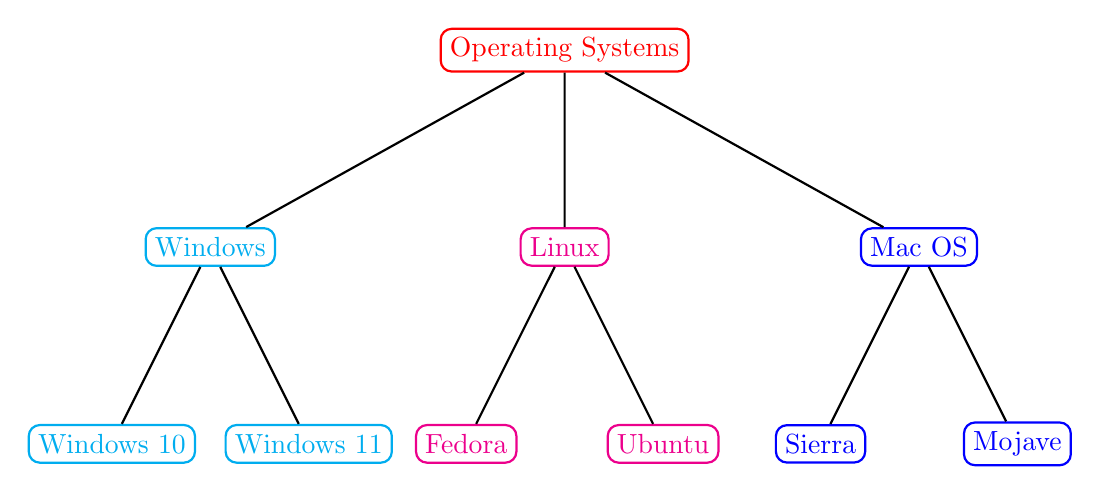
\begin{tikzpicture} [every node/.style = {shape=rectangle, rounded corners, draw, align=center}]
			\path [draw,thick,-]
			node (root)[red] {Operating Systems}
			[sibling distance=45mm, level distance=25mm]
			child {node [cyan] {Windows}
				[sibling distance=25mm, level distance=25mm]
				child { node [cyan] {Windows 10} }
				child { node [cyan] {Windows 11} }
			}
			child {node [magenta] {Linux}
				[sibling distance=25mm, level distance=25mm]
				child { node [magenta] {Fedora} }
				child { node [magenta] {Ubuntu} }
			}
			child {node [blue] {Mac OS}
				[sibling distance=25mm, level distance=25mm]
				child { node [blue]{Sierra} }
				child { node [blue]{Mojave} }
			};
		\end{tikzpicture}
	\caption{Operating Systems Family}
\end{figure}
\end{document}

